\chapter{Teoretický rozbor}

\section{Onemocnění covid-19}
\subsection{Popis onemocnění}

Covid-19 je vysoce nakažlivé onemocnění způsobené koronavirem SARS-CoV-2. Virus se šíří zejména vzdušnými kapénkami, které mohou být infikované, pokud je jedinec nakažený. Tyto kapénky můžeme vylučovat při dýchání, kašlání, mluvení nebo zpěvu. Existuje také možnost šíření viru kontaminovaným povrchem, ale to není hlavní cesta přenosu. Příznaky onemocnění covid-19 jsou různé a~mohou zahrnovat horečku, kašel, únavu, dýchací potíže, ztrátu čichu a~chuti. Mohou se také vyskytnout případy tzv. bezpříznakového průběhu, osoby s~takovým průběhem nevykazují žádné příznaky, ale mohou infekci šířit. U~každého jedince jsou příznaky individuální \cite{covid-info-gov}.

\subsection{Původ a~rozšíření nemoci}
Samotné první případy nemoci se datují v~prosinci 2019 v~čínském městě Wu-chan. Od té doby se virus rozšířil po celém světě rychlým tempem. Již 30. ledna 2020 vyhlásila Světová zdravotnická organizace (WHO) stav ohrožení veřejného zdraví mezinárodního významu a~později 11. března 2020 vyhlásila pandemii \cite{covid-19-who}. Pandemie se dotkla i~České republiky, kde se objevily první případy 1. března 2020, což vzbudilo pozornost českých občanů. Existuje několik teorií původu viru způsobující onemocnění covid-19, ale stále neexistuje přesné vysvětlení. Mnoho vědců se domnívá, že tento koronavirus je zoonotického původu (infekce přirozeně přenosné mezi zvířaty a~lidmi \cite{covid-19-zoonoza}) v~přirozeném prostředí a~že by mohl pocházet z~viru přenášeného netopýry. 

Někteří vědci a~politici se domnívali, že by SARS-CoV-2 mohl být náhodně uvolněn z~laboratoře. Tato teorie se ale zdá být méně pravděpodobná než ta, že je virus přírodního původu, protože doposud neexistují žádné relevantní důkazy, které by tuto teorii podpořily \cite{covid-19-origin}.

\subsection{Dopady pandemie}
Pandemie koronaviru je zdrojem různých negativních dopadů na českou ekonomiku. Jedním z~nejvíce zasažených sektorů českého hospodářství je cestovní ruch. Lidé kvůli probíhající pandemii omezili cestování. Jeho podíl na tvorbě hrubého domácího produktu země se propadl na 1,48 \% a~zaměstnanost v~tomto oboru se snížila o~7,3 \% \cite{dopady-covid-cestruch}. Cestovní ruch ve světě byl razantně omezen, v~roce 2021 byl zaznamenán propad turistických cest až o~85 \% oproti roku 2019. Když se počet zahraničních cest omezil, naopak stoupl počet delších tuzemských cest v~ČR až o~22 \% \cite{dopady-covid-cestruch-2}.

Během pandemie byl několikrát vyhlášen nouzový stav, jedná se o~takový krizový stav, který se vyhlašuje při vzniku různých nebezpečí, které ve značném rozsahu ohrožují životy, zdraví, majetkové hodnoty anebo vnitřní pořádek a~bezpečnost země \cite{dopady-covid-nouzstav}. V~tomto stavu platily různé zákazy a~omezení, všechna tato omezení platila různě dlouhou dobu, od několik dní až po několik týdnů. Mezi tato omezení patří například:

\begin{itemize}
    \item zákaz vycházení bez ochrany obličeje,
    \item zákaz provozu restaurací a~některých obchodů,
    \item zákaz veřejných i~soukromých akcí a~zákaz vstupu veřejnosti do sportovních a~kulturních zařízení,
    \item zákaz pobývat na veřejnosti v~počtu více než dvou osob.
\end{itemize}

Pokud byla u~vás zjištěna přítomnost koronaviru, museli jste být několik dní izolováni. Izolace byla nařízena osobám s~potvrzenou infekcí, což zahrnuje pozitivní výsledek testu na covid-19. Nařízení izolace vydává poskytovatel zdravotní péče nebo krajská hygienická stanice. Karanténa se vztahuje na osoby, které byly ve styku s~infikovanou osobou během inkubační doby onemocnění nebo pobývaly v~ohnisku nákazy. Cílem karantény je zabránit šíření infekčního onemocnění \cite{dopady-covid-izolace}. Při nedodržení karantény nebo izolace hrozily vysoké pokuty.

Proti koronaviru se dá v~současné době očkovat. Bez platného očkování byl v~minulosti např. zakázán vstup do sportovních, kulturních a~gastronomických zařízení anebo byl zakázán vstup do některých cizích zemí. Vakcíny proti covid-19, které jsou schválené EU, jsou velmi účinné v~ochraně před závažným průběhem onemocnění nebo úmrtím, a~to i~v~případech, kdy jsou způsobeny novými variantami viru SARS-CoV-2. Očkování však nezaručuje absolutní ochranu před nákazou covid-19. Jeho hlavním cílem je prevence vážných příznaků a~průběhů onemocnění \cite{dopady-covid-vakciny}.

\clearpage

\subsection{Současný stav}
Českou republikou se prohnalo několik covidových vln. Tyto vlny způsobily okamžitý růst počtu infikovaných osob onemocněním covid-19 a~zvýšily tlak na zdravotnická zařízení. V~současné době (duben 2023) je vliv koronaviru výrazně slabší, počet nově nakažených za den je mnohem nižší oproti minulosti, denně se nakazí v~průměru pár stovek lidí. Na obrázku \ref{fig:SoucasnyCovid} lze vidět vývoj počtu osob s~aktuálně probíhajícím onemocněním po celou dobu zaznamenávání dat o~koronaviru. Graf pochází z~webu MZČR, který je dostupný na \cite{onemocneni-aktualne}.

\begin{figure}[h]
	\centering
	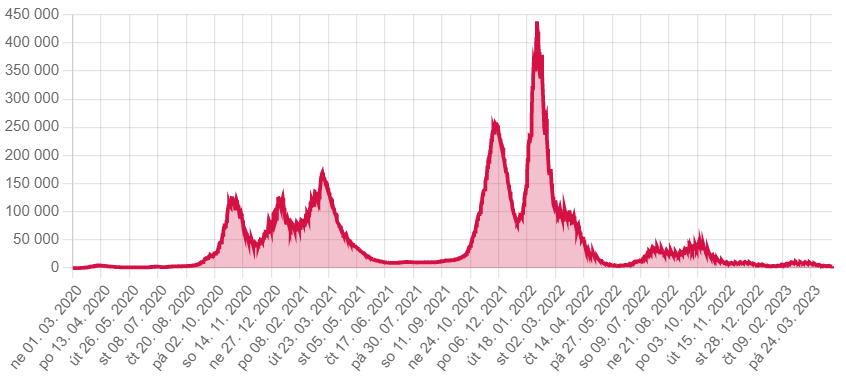
\includegraphics[width=1\textwidth]{Pictures/onemocneni.png}
	\caption{Přehled celkového počtu osob s~aktuálně probíhajícím onemocněním covid‑19\cite{onemocneni-aktualne}}
	\label{fig:SoucasnyCovid}
\end{figure}

Podle projektu OpenDataLab má ukončené očkování přes 6,8 miliónů lidí v~ČR, to činí přes 65\% obyvatel, celkový počet vydaných dávek přesahuje 18 miliónů. Celkový počet úmrtí v~ČR na toto onemocnění činí přes 42 tisíc \cite{soucasnystav-covid-statistika}.

Momentálně není v~České republice v~případě pozitivního výsledku testu automaticky nařizována karanténa. Izolace se nařizuje pouze v~situacích, kdy je to nutné pro zachování ochrany veřejného zdraví \cite{dopady-covid-izolace}. Omezení, která se vztahovala v~případě absence očkování, již neplatí. I~přesto, že již povinnost mít zakryté dýchací ústrojí respirátorem nebo rouškou není platná, stále se potkáte s~lidmi, kteří se pečlivě chrání.

\section{Současné aplikace}
\label{existing-apps}
Ministerstvo zdravotnictví poskytuje základní přehled o~dění v~souvislosti s koronavirem na svých online stránkách přes webovou aplikaci. Mimo jiné poskytuje i~webové API, které umožňuje vývojářům stahovat data.

\subsection{Webový portál MZČR}
MZČR má svůj vlastní webový portál na stránkách Onemocnění aktuálně \cite{onemocneni-aktualne}, který poskytuje informace o~stavu nemoci covid-19 v~České republice. Tento portál se nazývá Onemocnění aktuálně a~vznikl ve spolupráci s~ÚZIS ČR.

Ústav zdravotnických informací a~statistiky ČR je částí vlády, kterou zřizuje Ministerstvo zdravotnictví. ÚZIS ČR je správcem Národního zdravotnického informačního systému. Tento ústav spolupracuje s~Českým statistickým úřadem a~poskytovateli zdravotních služeb a~má vazby s~mnoha jinými zdravotnickými organizacemi jako jsou WHO, OECD, OSN a~EUROSTAT. Podle zákona je zdrojem oficiálních informací o~zdravotnické statistice pro Českou republiku \cite{uzis-definice}.

\subsubsection*{Hlavní stránka}

Hlavní stránka obsahuje přehled o~nemoci v~rámci celé ČR a~také řadu interaktivních grafů, které se dají měnit podle zvoleného časového rozmezí. Mezi informace, které grafy vyobrazují, patří např. přehled počtu osob s~nově prokázaným onemocněním covid-19 a~také přehled osob s~aktuálně probíhajícím onemocněním covid-19. Dále zde také najdete počty provedených PCR a~antigenních testů nebo i~přehled hospitalizací osob s~prokázaným onemocněním. Na hlavní stránce se nachází dvě interaktivní mapy, obě mapy vyobrazují výskyt laboratorně prokázaného onemocnění covid-19 s~tím rozdílem, že jedna z~nich zohledňuje kraje a~druhá okresy. Mapy vyobrazují jedinou informaci a~to celkový počet případů onemocnění za celé vaše zvolené období. 

\subsubsection*{Krajské zpravodajství}

Pokud bychom se chtěli dozvědět více informací o~krajích, webový portál nám umožňuje filtrovat data podle kraje. Na webové stránce se zvoleným krajem se vyskytují téměř totožné interaktivní grafy společně s podobnými přehledy, tentokrát pouze pro určitý kraj. Překvapí nás ale nové interaktivní mapy, v~tomto případě jsou dostupné tři a~mají rozšířenou funkčnost. I~přesto, že mapy vyobrazují celou ČR, tak se zobrazují hodnoty pouze v~okresech, které se nachází v~současně vybraném kraji. Tyto interaktivní mapy zobrazují denní přírůstky onemocnění, vyléčených osob a~také úmrtí. Barvy na mapě se škálují podle nejvyššího denního přírůstku v~rámci okresu za celé sledované období. Díky tomu lze na mapě spatřit tzv. covidové vlny. Má to ale i~svou nevýhodu, a~to, že mimo zmíněné covidové vlny jsou barvy na mapě těžce rozeznatelné. Bohužel nelze tyto mapy jinak přizpůsobit. Máme k~dispozici zvolení určitého dne a~spuštění animace, ale mapa nám nedovolí si zvolit určité období a~pohybovat se pouze v~daném období, tudíž by se nám barvy na mapě škálovaly odlišně. Proti tomuto se dá argumentovat, že by zobrazované hodnoty mohly být zkreslené, ale díky tomu můžeme naopak lépe pozorovat období mimo covidové vlny. Příklad mapy vyobrazující denní přírůstek onemocnění lze vidět na obrázku \ref{fig:OnemocneniAktualneScreen}.

\begin{figure}
	\centering
	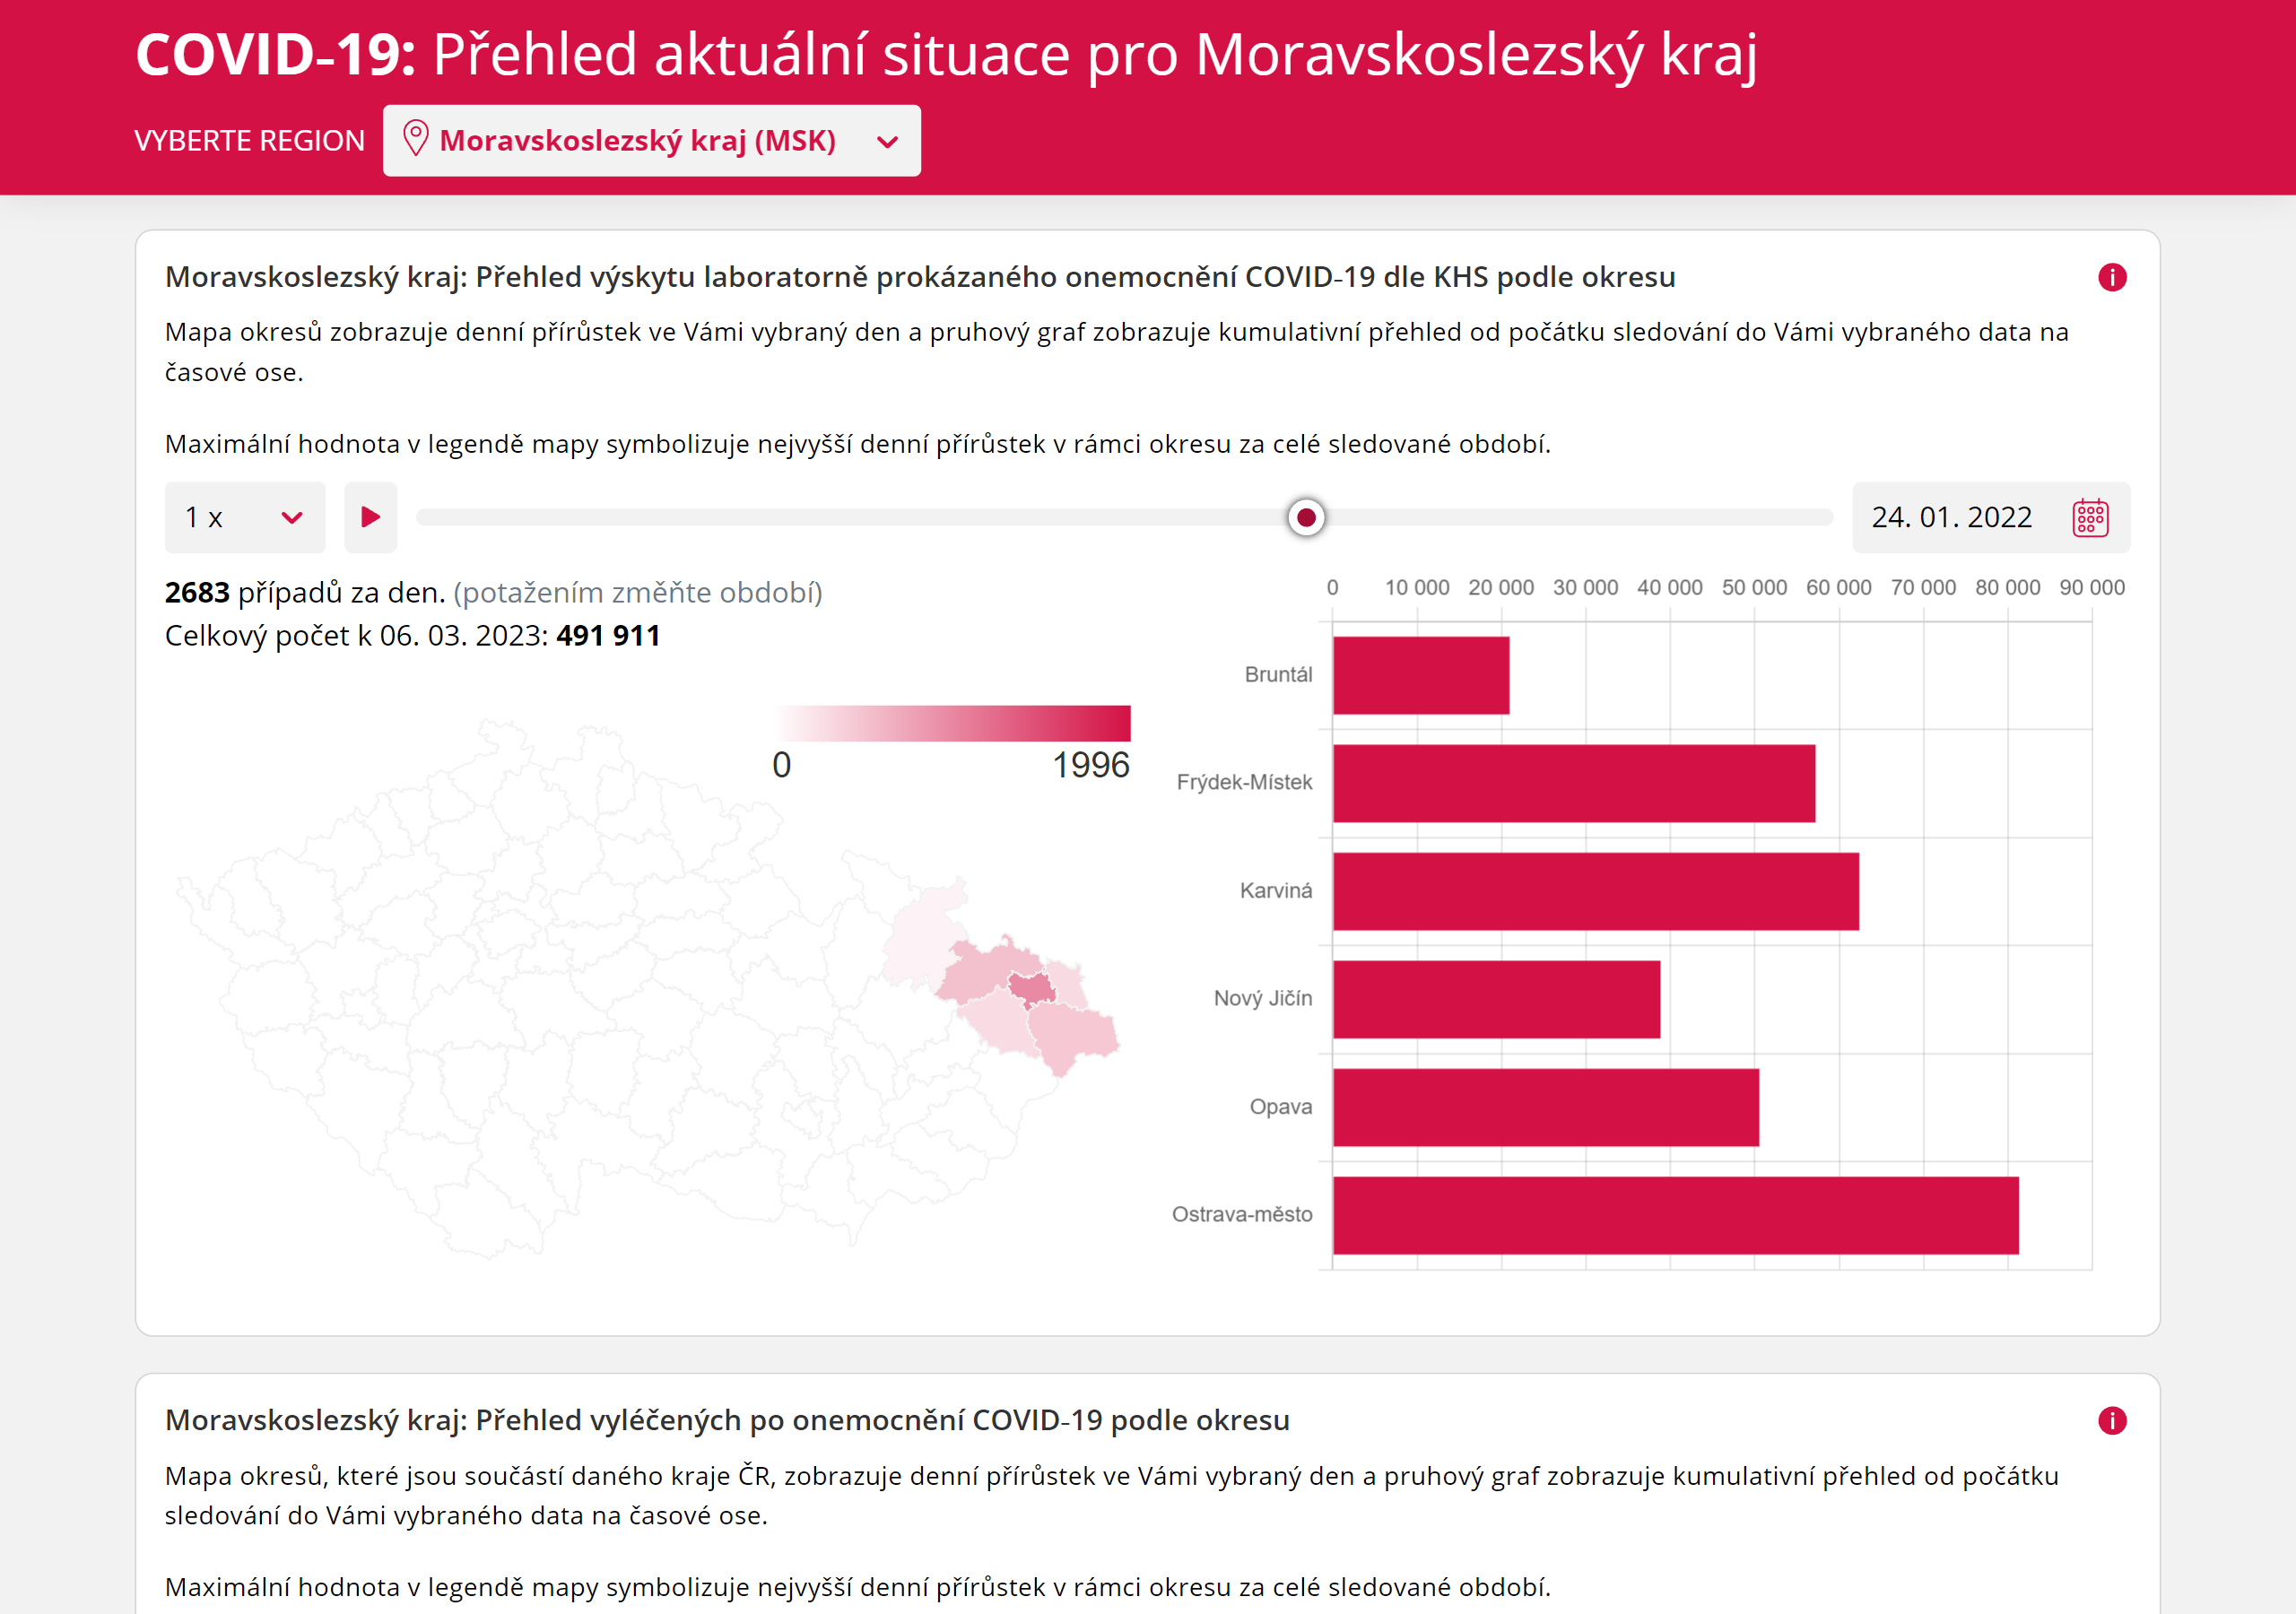
\includegraphics[width=0.8\textwidth]{Pictures/onemocneni-aktualne-screen.png}
	\caption{Vizualizace onemocnění v~aplikaci Onemocnění aktuálně v~Moravskoslezském kraji\cite{onemocneni-aktualne-msk}}
	\label{fig:OnemocneniAktualneScreen}
\end{figure}

\subsubsection*{Přehledy dle KHS}

Lepší přehled o~okresech lze nalézt v~záložce \emph{Přehledy dle KHS}. Na této stránce jsou funkčně totožné interaktivní mapy jako u~krajů s~tím rozdílem, že se na mapě ČR vyobrazují všechny okresy. Můžeme zkoumat data denních přírůstků infekcí, vyléčení a~úmrtí, ale stejně jako u~krajů si nemůžeme mapu nijak přizpůsobit. Opět se barvy na mapě škálují podle nejvyššího denního přírůstku v~rámci okresu za celé sledované období.

Ideální interaktivní mapa by zobrazovala všechny okresy na jedné mapě ČR s~možnostmi přizpůsobení období a~škálování, takovou mapu v~této webové aplikaci nenajdeme.

\subsection{OpenDataLab}
Projekt OpenDataLab vznikl ve spolupráci s~Fakultou informačních technologií ČVUT v~Praze a~společností Profinit EU. Jedná se o~otevřenou laboratoř určenou hlavně pro studenty. Jejich hlavním cílem je nabídnout nápady, pomoc a~případně i~zadání semestrálních a~závěrečných prací studentům, jejich práce vytvořené pro školu jsou veřejné a~slouží k~dobrému účelu \cite{opendatalab}.

Jedním z~jejich realizovaných projektů je web poskytující především statistická data o~jednotlivých očkovacích místech, jejich dostupnosti, zaplněnosti a~celkových statistikách o~daném místě. Očkovací místa se dají roztřídit podle krajů nebo typu vakcíny, takže se v~datech neztratíte. Aplikace také umožňuje místa filtrovat detailněji, např. podle věku, zda je nutno se na daném místě registrovat nebo zda je dané místo i~pro samoplátce. U~každého očkovacího místa se dozvíte kolik lidí je právě rezervovaných a~u~některých se i~dozvíte průměrnou dobu čekání na rezervaci.

Mimo vyhledávání očkovacích míst zahrnuje tento web souhrnné statistiky o~koronaviru a~očkování v~ČR. Na této stránce vás uvítá rozsáhlá tabulka dat, která zahrnuje mnoho informací o~očkování např. počtu rezervací na očkování, vydaných dávek nebo počet lidí čekajících ve frontě. 

\begin{figure}[h]
	\centering
	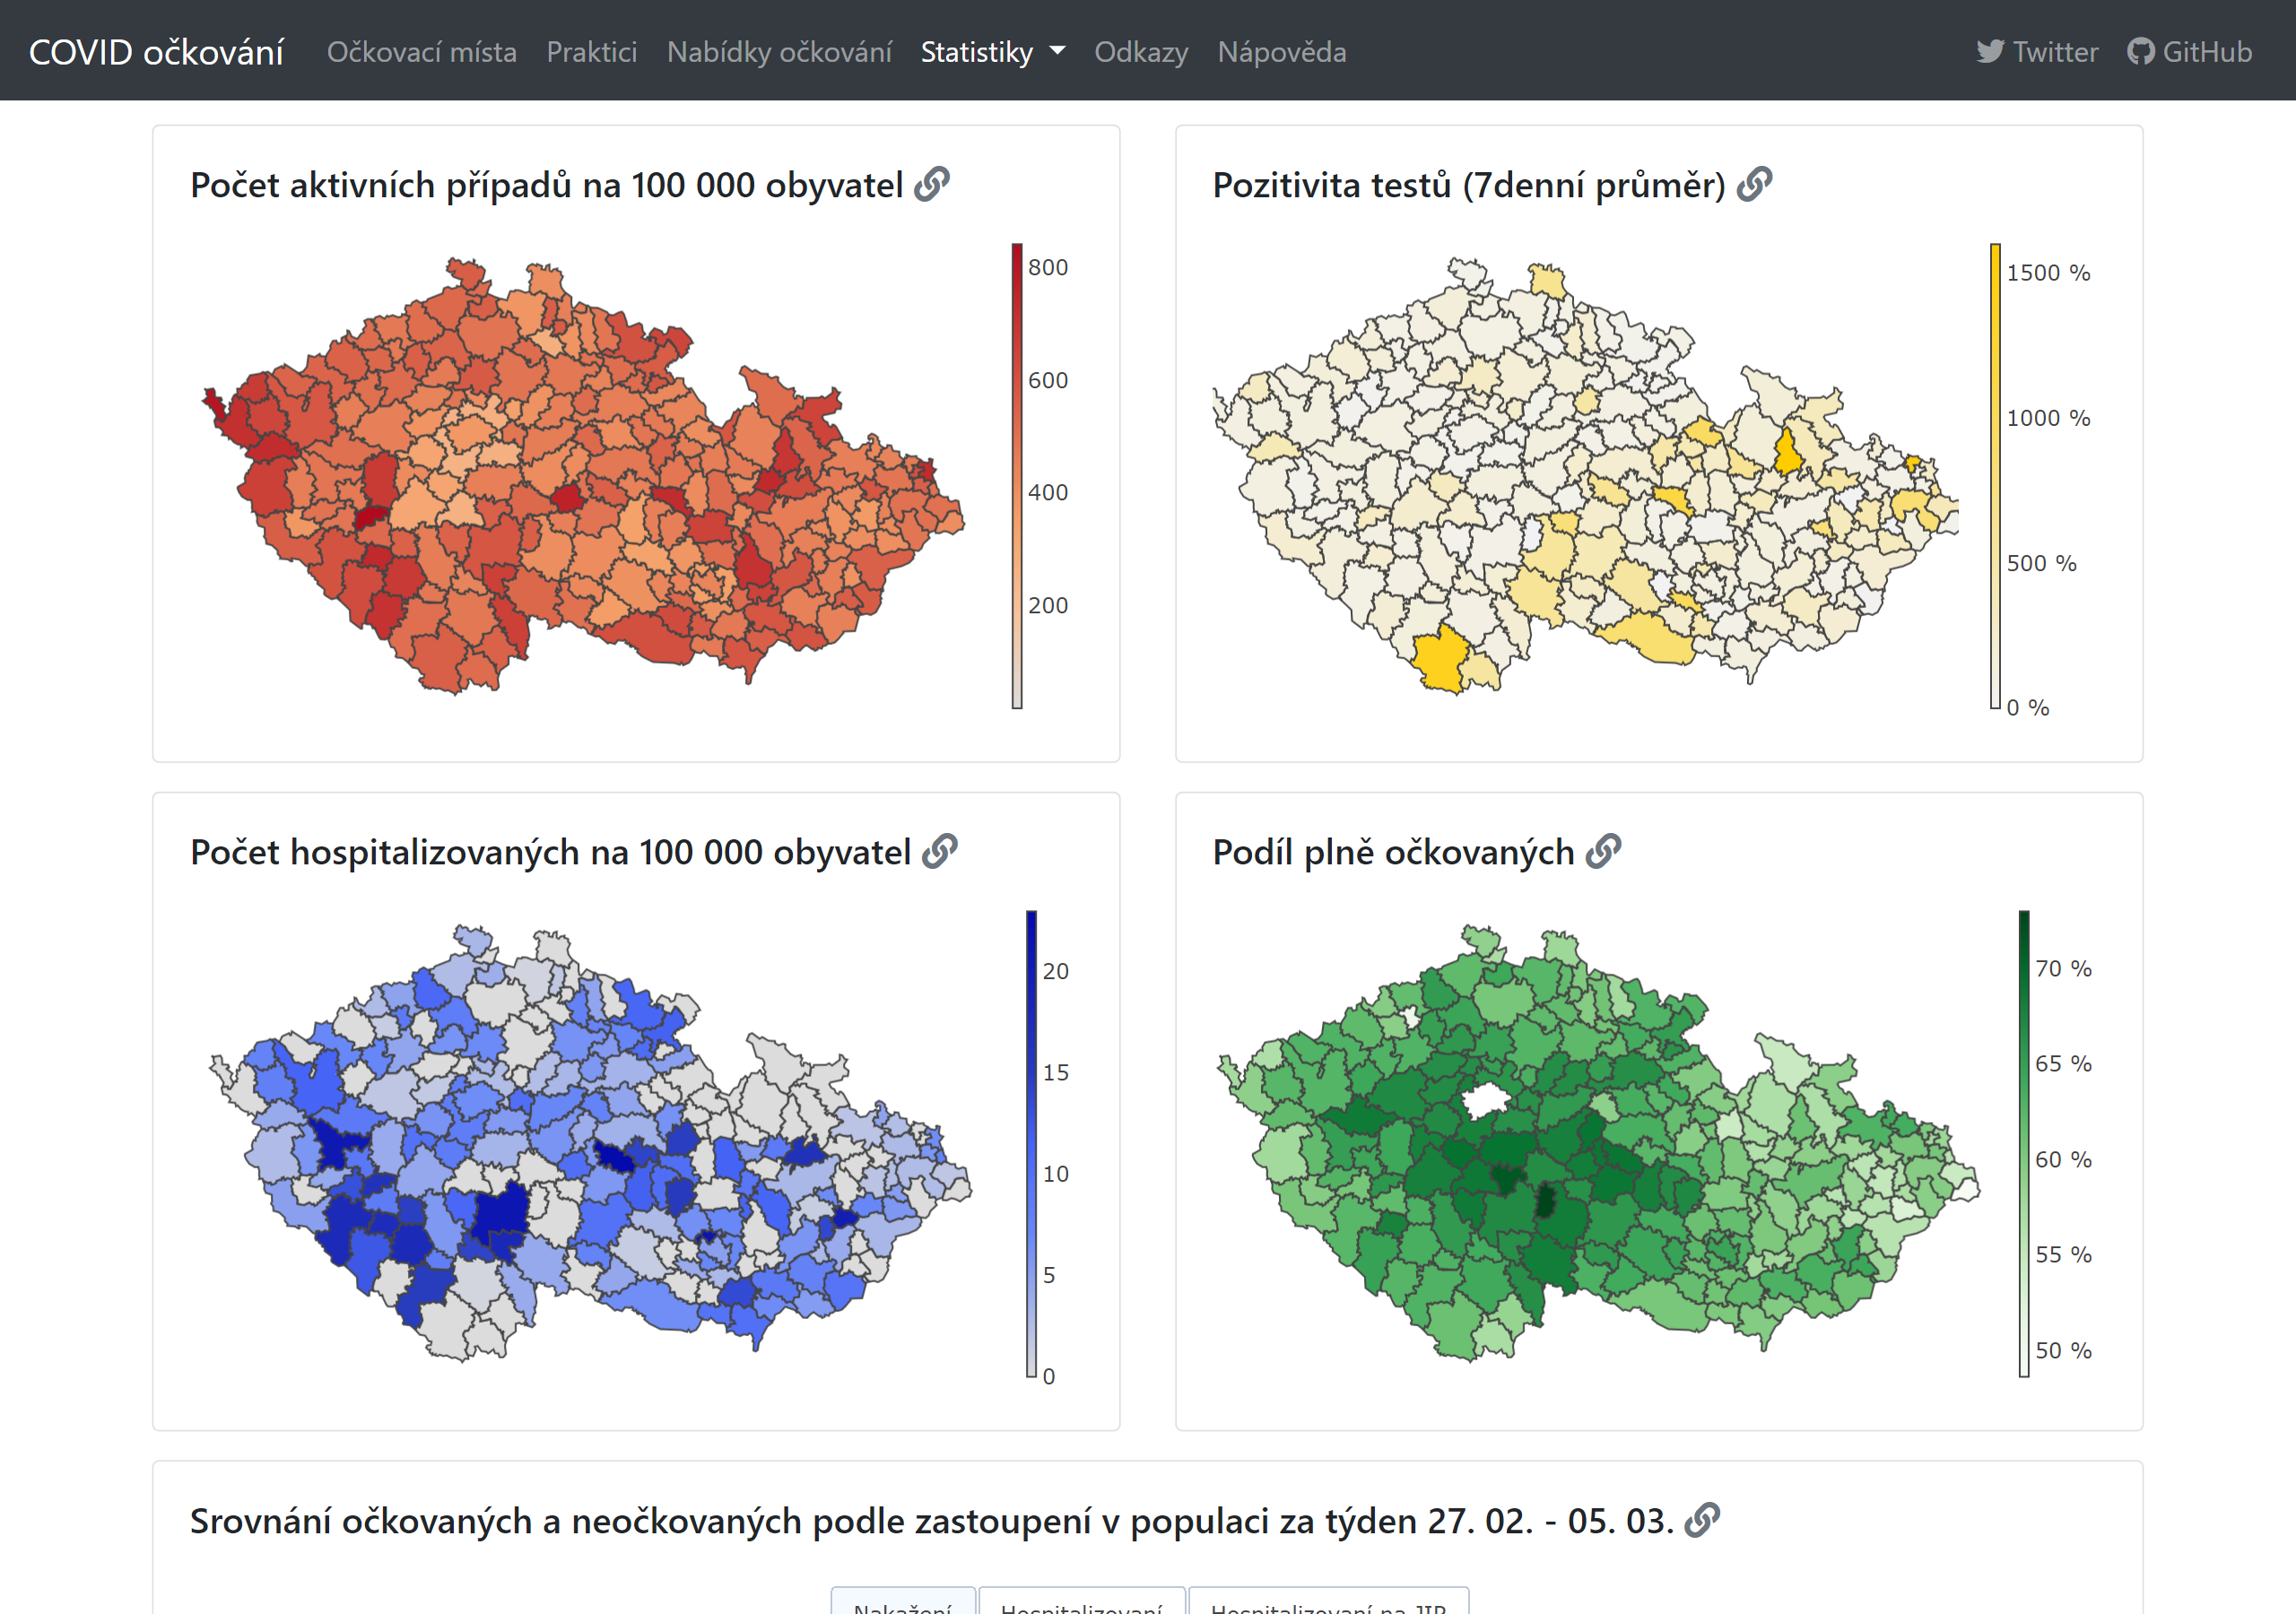
\includegraphics[width=1\textwidth]{Pictures/opendatalab-screen.png}
	\caption{Vizualizace onemocnění v~aplikaci projektu OpenDataLab \cite{soucasnystav-covid-statistika}}
	\label{fig:OpenDataLabScreen}
\end{figure}

Součástí statistik jsou i~souhrnné mapy, které vyobrazují současný stav z~hlediska aktivních případů, pozitivity testů, počtu hospitalizovaných a~plně očkovaných. Tyto mapy nejsou nijak přizpůsobitelné a~nelze si je omezit na určité období. Nejdůležitější část této statistiky jsou interaktivní grafy, které jsou zaměřené na vývoj počtu očkovaných, registrací, front a~nebo také na porovnání různých typu vakcín. Zmíněné mapy lze spatřit na obrázku \ref{fig:OpenDataLabScreen}.

Tuto webovou aplikaci lze nalézt na stránkách OpenDataLab \cite{opendatalab-ockovani}.

\section{Dostupná data}

\subsection{O~dostupných datech}
Data o~počtech ovlivněných koronavirovým onemocněním mohou být získávána z~různých zdrojů. WHO (\emph{World Health Organization}) poskytuje data na celosvětové úrovni, ECDC (\emph{European Centre for Disease Prevention and Control}) pro Evropu a~CDC (\emph{Centers for Disease Control and Prevention}) pro Spojené státy americké. V~rámci jednotlivých zemí poskytují regionální data ministerstva zdravotnictví. V~ČR jsou data dostupná veřejnosti v~datových sadách, které spravuje MZČR \cite{bednarkova-covid}.

\subsection{Onemocnění aktuálně API v3}
\label{sec:onemocneni-aktualne}
Součástí webového portálu Onemocnění aktuálně jsou i~otevřené datové sady zdarma ke stažení obsahující širokou škálu dat o~onemocnění covid-19. Existuje několik verzí těchto datových sad, starší verze jsou zprostředkovány jako rozsáhlé datasety ve formě CSV. Pracovat budeme s~nejnovější verzí 3, která je zprostředkována jako webové API.

API je zkratkou pro aplikační programovací rozhraní. Jedná se o~rozhraní, které poskytuje řadu funkcí, jež umožňují programátorovi přistoupit k~určitým datům nebo funkcím aplikace. V~podstatě se jedná o~způsob, jakým aplikace mezi sebou komunikují, aby mohly sdílet data a~funkce \cite{api-definice}. Webové API je takové API, ke kterému je možné přistoupit prostřednictvím webu.

K~dispozici je široká škála dat, avšak pouze část těchto dat zohledňuje okresy ČR. Zde je seznam datasetů, které byly využity při tvorbě aplikace, a jaká data byla z těchto datasetů použita:
\begin{itemize}
    \item \emph{obce} (informace o~případech infekce v~obcích),
    \item \emph{ockovani-geografie} (informace o~vydaných dávkách očkování v~krajích s~bydlišti osob na úrovni ORP),
    \item \emph{umrti} (informace o~nových úmrtí v~okresech),
    \item \emph{kraj-okres-testy} (informace o~provedených PCR testech v~okresech).
\end{itemize}

Všechny zmíněné datasety kromě \emph{ockovani-geografie} obsahují informace na úrovni okresů. Pouze u~datasetu \emph{ockovani-geografie} je potřeba zařadit ORP do okresu. Dataset obsahuje informace o~vydaných dávkách očkování v~daném kraji s~bydlištěm očkované osoby na úrovni ORP. Aplikace tudíž bude vyobrazovat počet vydaných dávek na základě bydlišť osob, takže vyobrazené informace nemusí být zcela přesné.

Je důležité zmínit, že poskytovaná data se neustále mění. Dochází tak k~nepřesnostem při snaze zvizualizovat brzká data, proto je doporučeno 
se na tato data nespoléhat a~vyčkat několik dní nebo i~týdnů, než se data zaktualizují na přesnější hodnoty.

Každý záznam poskytovaný tímto API má přiřazený svůj identifikační řetězec, pomocí kterého se dá nalézt a~získat určitý záznam. Veškerá dokumentace k~tomuto API je dostupná na stránkách Onemocnění aktuálně \cite{onemocneni-aktualne-docs}.

\subsubsection*{Získání dat}

Data jsou volně přístupná komukoli, jediným požadavkem je registrace na portálu Onemocnění aktuálně. Po registraci získáte vlastní token, pomocí kterého je komunikace s~API zabezpečena. Token je při komunikaci s~API potřebný, při pokusu o~komunikaci bez tokenu vám API žádná covidová data nevrátí, pouze vás upozorní na absenci tokenu.

Pro získání dat z~API MZČR je potřeba zaslat dotaz na API ve formě HTTP požadavku. Požadavek musí obsahovat platný token a~také platnou URL adresu, která definuje typ žádaných dat. URL adresa může obsahovat různé parametry, např. omezení počtu výsledků, číslo stránky, omezení časového rozsahu nebo zvolení konkrétního okresu. Limit počtu dotazů každého uživatele je stanoven na 1000/hod. V~kódu \ref{src:PythonListing} je příklad pro získání dat z~API v~jazyce Python, přesněji získání kumulativních počtů souvisejících s~nemocí v~okrese Ostrava-město dne 5. ledna 2023:


\begin{lstlisting}[language=Python,label=src:PythonListing,caption={Zaslání HTTP požadavku v~jazyce Python}]
from urllib import request

url = 'https://onemocneni-aktualne.mzcr.cz/api/v3/kraj-okres-nakazeni-vyleceni-umrti?page=1&itemsPerPage=100&datum%5Bbefore%5D=2023-01-05&datum%5Bafter%5D=2023-01-05&okres_lau_kod=CZ0806&apiToken=xyz'
req = request.Request(url)
req.add_header('accept', 'application/json')
response = request.urlopen(req)

\end{lstlisting}

\subsubsection*{Formát dat}
API verze 3 nám umožňuje vyžádat si různý formát dat výsledku. Hodnotu výsledku to neovlivní, pouze se změní formátování vráceného dokumentu. Pro vyžádání určitého formátu stačí do HTTP požadavku vložit hlavičku \emph{accept} s~hodnotou daného formátu. K~dispozici máme čtyři možnosti:

\begin{itemize}
    \item application/ld+json (formát JSON-LD),
    \item application/json (formát JSON),
    \item text/html (formát HTML),
    \item text/csv (formát CSV).
\end{itemize}

Příklad formátování je k~dispozici v~kódu \ref{src:JavaListing}, kde se nachází vrácený výsledek Python kódu \ref{src:PythonListing} s~vyžádaným formátem application/json:

\begin{lstlisting}[language=Java,label=src:JavaListing,caption={Příklad vráceného výsledku API}]
[
  {
    "id": "8ed855a3-35c6-40c3-8a8f-7cf4ddd169d5",
    "datum": "2023-01-05",
    "kraj_nuts_kod": "CZ080",
    "okres_lau_kod": "CZ0806",
    "kumulativni_pocet_nakazenych": 131424,
    "kumulativni_pocet_vylecenych": 130766,
    "kumulativni_pocet_umrti": 1434
  }
]

\end{lstlisting}

Vrácená data jsou ve vyžádaném JSON formátu, s~tímto formátem bude aplikace pracovat. JSON je zkratka pro \emph{Java Script Object Notation}, jedná se o~odlehčený formát pro výměnu dat, který je snadno srozumitelný. JSON je textový formát, který je zcela nezávislý na jazyku, ale používá konvence, které jsou známé programátorům jazyků jako jsou C++, C\#, Java, JavaScript, Python a~mnoho dalších \cite{json-definice}.

Při požádání o~data nám toto API vrátí výsledek, který je sestupně setřízený podle dní. Pokud obsahuje výsledek i~identikační kódy, jako např. NUTS kód nebo LAU kód, bývá tento výsledek sestupně setřízený i~podle těchto kódů.

\subsection{Pomocná data ČSÚ}
\label{csu}
Při práci s~daty ÚZIS a~MZČR budou potřeba dodatečná data, která jsou dostupná online na stránkách Českého statistického úřadu. Bude potřeba identifikovat okresy a~obce podle jejich identifikačních kódů, zařadit ORP do okresů a~také bude potřeba znát počty obyvatel v~okresech pro přepočty hodnot.

\subsubsection*{Seznam okresů a~jejich identifikace}

Pokud žádáme zmíněné API o~data, která jsou spojena s~kraji, okresy nebo obcemi, obsahují tato data identifikátory, které definují o~jaký územní celek se jedná. MZČR pracuje ve svém API s~identifikačními NUTS kódy a~LAU kódy.

Klasifikace NUTS (\emph{Nomenclature of territorial units for statistics}) je systém, který slouží k~rozdělení ekonomického území Evropské unie a~Spojeného království na různé úrovně. Cílem tohoto systému je získávat statistická data a~socioekonomické informace o~jednotlivých regionech. Klasifikace NUTS obsahuje více úrovní, které umožňují podrobnější rozdělení regionů:

\begin{itemize}
    \item NUTS 1: nejvyšší úroveň regionů - celé území ČR,
    \item NUTS 2: regiony druhé úrovně - regiony (např. Moravskoslezsko, Střední Čechy nebo Jihovýchod),
    \item NUTS 3: malé regiony - kraje ČR \cite{europa-eu-nuts}.
\end{itemize}

LAU (\emph{Local administrative unit}) je systém, který byl vytvořený EU pro identifikaci územních jednotek v~Evropě. Oproti NUTS, který se používá na regionální evropské úrovni, se LAU používá na místní úrovni. Používá se také pro statistické účely jako např. pro sběr a~analýzu dat v~oblastech demografie, hospodářství a~jiné. Tyto jednotky se považují za stavební jednotku NUTS systému a~v~ČR se řadí do dvou úrovní:

\begin{itemize}
    \item horní úroveň LAU 1 - okresy,
    \item spodní úroveň LAU 2 - obce \cite{csu-lau}.
\end{itemize}

Rozdělení České republiky na NUTS 3 (kraje) a~LAU 1 (okresy) lze vidět na obrázku \ref{fig:NutsLau}. Obrázek pochází z~webu ČSÚ \cite{nuts-lau-pic}.

\begin{figure}[h]
	\centering
	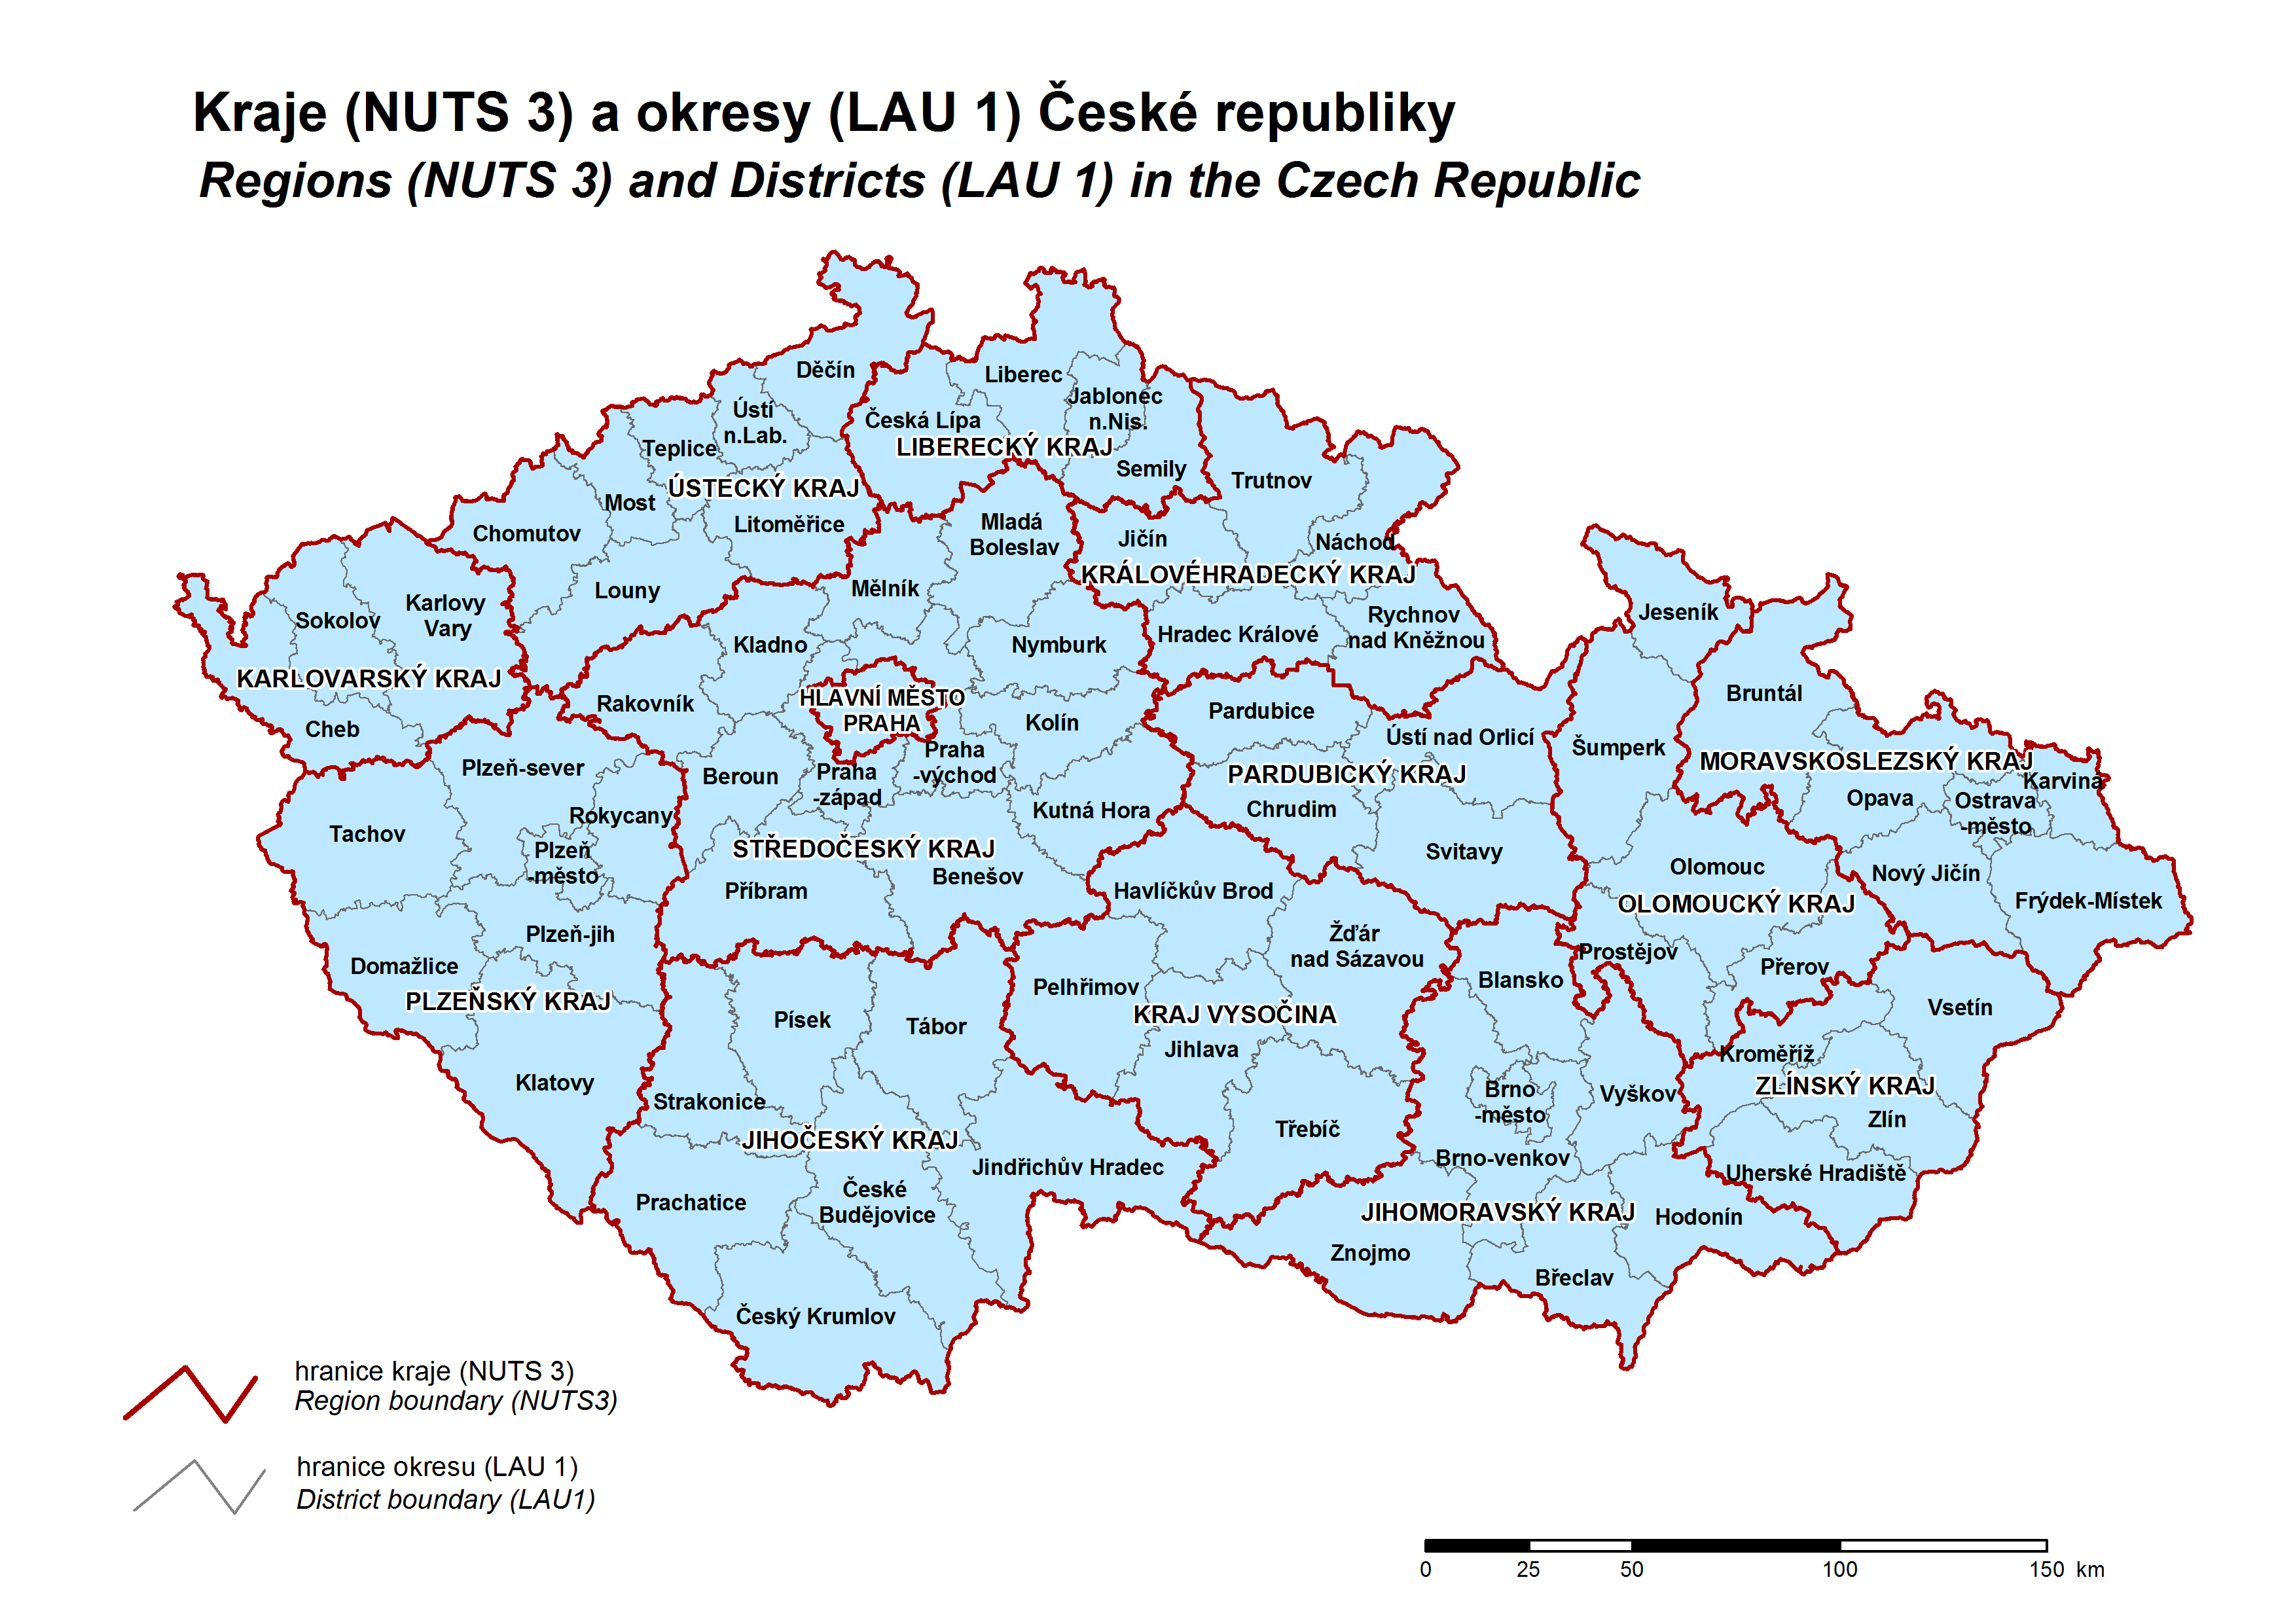
\includegraphics[width=1\textwidth]{Pictures/nuts_lau.png}
	\caption{Rozdělení České republiky na NUTS 3 a~LAU 1 \cite{nuts-lau-pic}}
	\label{fig:NutsLau}
\end{figure}

Vzhledem k~tomu, že je práce zaměřena na okresy ČR, budou se využívat pouze LAU kódy. Abychom mohli ve výsledcích API rozpoznat o~který okres se jedná, potřebujeme číselník, který nám umožní identifikovat daný LAU kód. Český statistický úřad poskytuje tento číselník online na stránkách ČSÚ \cite{czso-ciselnik-lau}. Číselník je možné stáhnout v~několika formátech, např. v~XML nebo CSV.

\subsubsection*{Zařazení ORP do okresů}
\label{sec:ciselnik-orp}

Práce bude využívat dataset s~informacemi o~vydaných dávkách očkování. Obsažená data nesou informaci o~bydlišti osoby, které byla vydaná jedna z~dávek. Bydliště je na úrovni ORP (obec s~rozšířenou působností) a~je nutné ji přiřadit okres, ve kterém se nachází. To umožní číselník na stránkách ČSÚ \cite{csu-ciselnik-orp}, který obsahuje potřebné informace k~přiřazení ORP do okresů.

\subsubsection*{Počet obyvatel v~okresech}

Při vizualizaci dat se bude pracovat i~s~přepočtem na sto tisíc obyvatel, který se běžně používá ve statistice. Jedná se o~hodnotu, která může přesněji vyobrazit situaci v~daném okrese. ČSÚ poskytuje své výsledky sčítání lidu na svých stránkách \cite{czso-pocet-obyvatel}. Data poskytuje ve formátu CSV a~obsahují velkou řadu informací, obsahuje nejen počty obyvatel v~krajích a~okresech rozdělené podle pohlaví, ale třeba i~průměrný věk podle pohlaví v~těchto celcích. Data byla přeformátována tak, aby byla jednoduše použitelná v~naší aplikaci.

\endinput